\label{sec:failure_analysis}

To understand systematic LLM failures in RetailBench, we analyze agent behavior through four operational diagnostics: \textit{product candidate selection}, \textit{evidence acquisition}, \textit{action conversion}, and \textit{temporal follow-up}. Together, these diagnostics capture the core operational loop of retail management: selecting products to manage, acquiring decision-relevant evidence, translating evidence into actions, and revisiting delayed consequences.

The diagnostics reveal three recurring failure patterns:
\begin{itemize}[leftmargin=*]
    \item \textbf{Incomplete evidence acquisition.} Agents often act on incomplete evidence, missing critical information for orders or price updates even when the corresponding tools are available.
    \item \textbf{Weak evidence-to-action conversion.} Agents rely on surface-level signals such as supplier price, while underweighting less visible but consequential factors such as supplier quality, product returns, expiration risk, and long-term profitability.
    \item \textbf{Lack of a consistent long-horizon policy.} Agents fail to maintain attention over important products and often do not follow up on delayed consequences of prior actions.
\end{itemize}
Detailed metric definitions are provided in Appendix~\ref{appendix:stage_metrics}.

\begin{figure*}[t]
    \centering

    \begin{minipage}{0.48\textwidth}
        \centering
        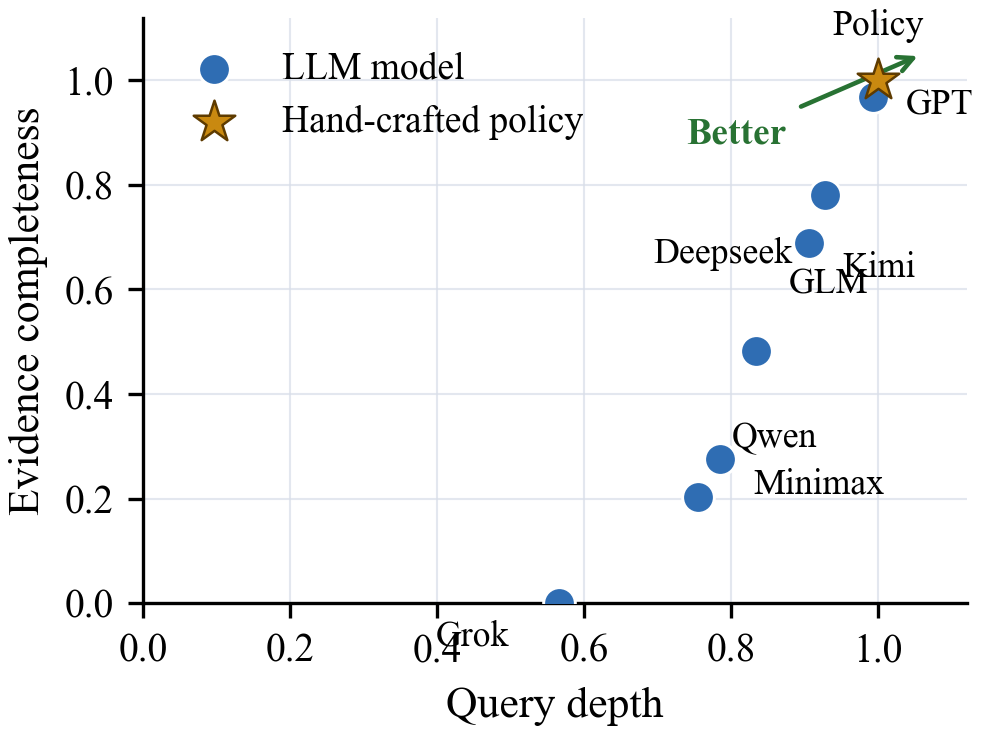
\includegraphics[width=\linewidth]{figures/stage2_evidence_single.png}
        \vspace{-0.5em}
        \centerline{\small \textbf{(a) Evidence acquisition}}
    \end{minipage}
    \hfill
    \begin{minipage}{0.48\textwidth}
        \centering
        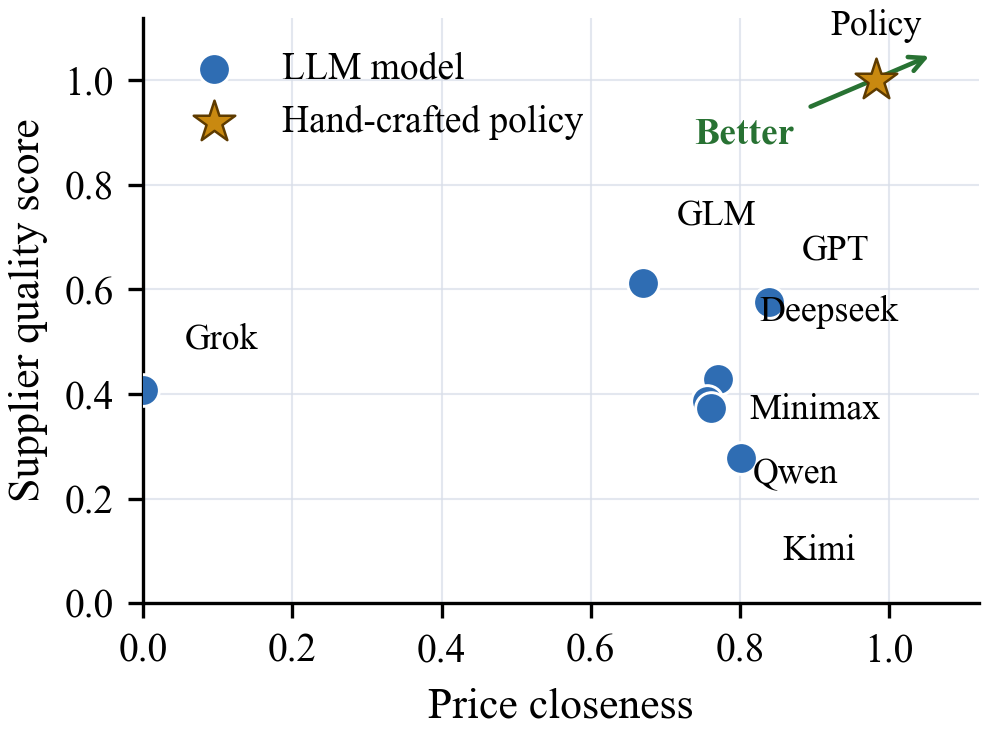
\includegraphics[width=\linewidth]{figures/stage3_action_single.png}
        \vspace{-0.5em}
        \centerline{\small \textbf{(b) Action conversion}}
    \end{minipage}

    \vspace{0.6em}

    \begin{minipage}{0.48\textwidth}
        \centering
        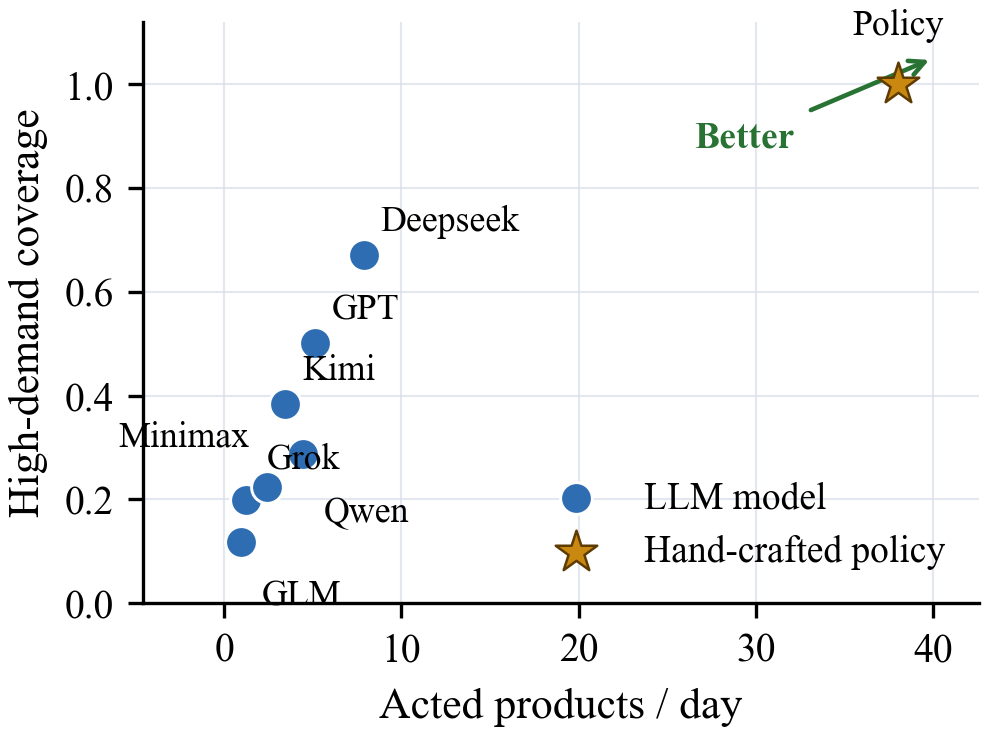
\includegraphics[width=\linewidth]{figures/stage1_sku_selection_single.png}
        \vspace{-0.5em}
        \centerline{\small \textbf{(c) Product candidate selection}}
    \end{minipage}
    \hfill
    \begin{minipage}{0.48\textwidth}
        \centering
        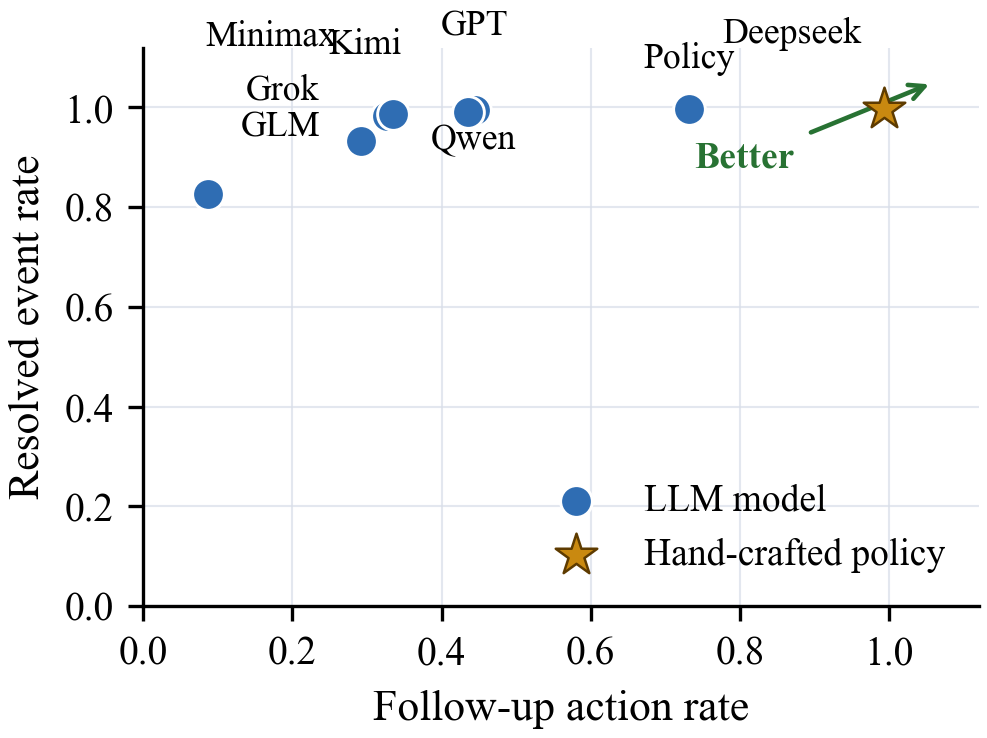
\includegraphics[width=\linewidth]{figures/stage4_followup_single.png}
        \vspace{-0.5em}
        \centerline{\small \textbf{(d) Temporal follow-up}}
    \end{minipage}

    \caption{Diagnostic analysis of the three failure patterns in RetailBench. Blue circles denote survival-first selected LLM runs, and the black star denotes the hand-crafted policy. Better performance appears toward the upper-right region in each panel. Panels (a) and (b) diagnose incomplete evidence acquisition and surface-level decision making, respectively; panels (c) and (d) diagnose the lack of a consistent long-horizon policy.}
    \label{fig:failure_diagnostics}
\end{figure*}

\subsection{Incomplete Evidence Acquisition}

The first failure pattern is incomplete evidence acquisition. Agents often place orders or update prices without inspecting key information about demand, inventory, supplier conditions, reviews, and external events. We use two diagnostics:
\begin{itemize}[leftmargin=*]
    \item \textbf{Query depth} ($\uparrow$): the fraction of required evidence categories queried before an order or price update.
    \item \textbf{Evidence completeness} ($\uparrow$): the fraction of actions for which all decision-critical evidence categories have been queried before execution.
\end{itemize}

Figure~\ref{fig:failure_diagnostics}(a) shows large variation in evidence acquisition. GPT-5.5 performs best, with a query depth of 0.9922 and an evidence completeness of 0.9689. DeepSeek-V4-Pro and Kimi-K2.6 also achieve high query depth, at 0.9279 and 0.9052, respectively. In contrast, MiniMax-M2.5, Qwen3.5, and Grok-4.3 show lower evidence completeness, with Grok-4.3 reaching 0.0000. This pattern broadly aligns with Table~\ref{tab:selected_main_results}, where agents with stronger evidence acquisition generally obtain better long-horizon outcomes. The result suggests that weakly structured evidence acquisition limits downstream action quality, though evidence collection alone does not guarantee effective decisions.

\subsection{Surface-Level Decision Making}

The second failure pattern is surface-level decision making. Agents often rely on immediately visible signals rather than criteria that determine long-term outcomes. In RetailBench, supplier price is directly observable, whereas supplier quality is only indirectly reflected through return rates and customer reviews. As a result, agents may favor low-cost suppliers even when lower quality can increase returns, weaken customer feedback, and reduce long-term profitability.

We use two diagnostics:
\begin{itemize}[leftmargin=*]
    \item \textbf{Price closeness} ($\uparrow$): the distance between the chosen price and an estimated historical-profit optimum.
    \item \textbf{Supplier quality score} ($\uparrow$): a rank-based quality score of the selected supplier among same-product candidates.
\end{itemize}

Figure~\ref{fig:failure_diagnostics}(b) shows that action conversion is the clearest bottleneck. The hand-crafted policy achieves a mean price distance of 1.98\% and an average supplier quality rank of 1.00. Among selected LLM runs, GPT-5.5 has the smallest price distance, 17.92\%, while supplier selection remains consistently weak: selected LLM mean quality ranks range from 2.55 to 3.89, and the best selected-run \textbf{QualityFirst} rate is only 34.65\%. Here, \textbf{QualityFirst} denotes choosing the raw-quality-best supplier among same-product candidates, whereas \textbf{PriceFirst} denotes choosing the cheapest supplier; Appendix~\ref{appendix:stage_metrics} and Figure~\ref{fig:supplier_selection_diagnostic} provide the detailed diagnostic definition and comparison. Across all LLM runs, \textbf{QualityFirst} is 21.5\%, compared with 55.6\% for \textbf{PriceFirst}.

Thus, the bottleneck is not merely tool use, but evidence-to-action reasoning. Agents often query supplier prices, yet less consistently query or use supplier-quality proxies, limiting their ability to make quality-adjusted decisions with better long-term outcomes.
\subsection{Lack of Consistent Long-Horizon Policy}

The third failure pattern is the lack of a consistent stateful policy over long horizons. Long-horizon store operation is not a sequence of independent daily decisions: agents must maintain attention over important products, track prior actions, and update procurement, shelf, and pricing decisions after delayed feedback arrives. We diagnose this pattern from two complementary perspectives: product candidate selection and temporal follow-up.

For product candidate selection, we use two diagnostics:
\begin{itemize}[leftmargin=*]
    \item \textbf{Acted products per day} ($\uparrow$): the average number of products receiving information queries or management actions, such as orders or price updates, per day.
    \item \textbf{High-demand coverage} ($\uparrow$): the extent to which daily top-sales or stockout products receive attention.
\end{itemize}

Figure~\ref{fig:failure_diagnostics}(c) shows insufficient product-level attention across LLM agents. The hand-crafted policy acts on 38.00 products per day and misses no retrospective high-demand opportunities. Selected LLM runs, however, act on only 0.95 to 7.89 products per day and miss 32.86\% to 88.18\% of high-demand opportunities. Even the strongest selected LLM on this diagnostic, DeepSeek-V4-Pro, acts on only 7.89 products per day and misses 32.86\% of high-demand opportunities.

These results indicate that many failures arise before action quality is considered: although daily sales may span more than 30 distinct products, most sold products simply do not enter the daily action set. Persistent narrowness in product attention reflects weak portfolio-level management, rather than a one-step action error.

For temporal follow-up, we use two diagnostics:
\begin{itemize}[leftmargin=*]
    \item \textbf{Follow-up action rate} ($\uparrow$): the fraction of acted products that receive another action within seven days.
    \item \textbf{Resolved-event rate} ($\uparrow$): one minus the rate of stockout, return, or expiration events left without later attention.
\end{itemize}

Figure~\ref{fig:failure_diagnostics}(d) shows substantial variation in follow-up quality. The hand-crafted policy follows up on 0.9936 of acted products within seven days and leaves only 0.0040 of delayed events unresolved. DeepSeek-V4-Pro has the strongest selected-LLM follow-up action rate, 0.7316, and an unresolved-event rate of 0.0028, consistent with its 180-day survival. GPT-5.5 also keeps unresolved events low at 0.0042, but its follow-up action rate is lower at 0.4443.

Together, product selection and temporal follow-up show that long-horizon failures are not merely poor one-step decisions. Agents lack persistent stateful policies that maintain product attention, revisit delayed consequences, and revise operational decisions after feedback arrives. This explains why some agents make occasional reasonable local decisions but still fail to sustain stable store operation over the full horizon.

Overall, systematic LLM failure in RetailBench arises from three interacting bottlenecks: incomplete evidence acquisition, weak evidence-to-action conversion, and inconsistent long-horizon policy. Improving long-horizon LLM agents therefore requires more than increased tool use; it also requires better evidence selection, deeper evidence-to-action reasoning, and more reliable stateful decision policies.
\FloatBarrier
